%-----------------------------------------------------------------------------------------------------------------------------------------------%
%	The MIT License (MIT)
%
%	Copyright (c) 2015 Jan Küster
%
%	Permission is hereby granted, free of charge, to any person obtaining a copy
%	of this software and associated documentation files (the "Software"), to deal
%	in the Software without restriction, including without limitation the rights
%	to use, copy, modify, merge, publish, distribute, sublicense, and/or sell
%	copies of the Software, and to permit persons to whom the Software is
%	furnished to do so, subject to the following conditions:
%
%	THE SOFTWARE IS PROVIDED "AS IS", WITHOUT WARRANTY OF ANY KIND, EXPRESS OR
%	IMPLIED, INCLUDING BUT NOT LIMITED TO THE WARRANTIES OF MERCHANTABILITY,
%	FITNESS FOR A PARTICULAR PURPOSE AND NONINFRINGEMENT. IN NO EVENT SHALL THE
%	AUTHORS OR COPYRIGHT HOLDERS BE LIABLE FOR ANY CLAIM, DAMAGES OR OTHER
%	LIABILITY, WHETHER IN AN ACTION OF CONTRACT, TORT OR OTHERWISE, ARISING FROM,
%	OUT OF OR IN CONNECTION WITH THE SOFTWARE OR THE USE OR OTHER DEALINGS IN
%	THE SOFTWARE.
%-----------------------------------------------------------------------------------------------------------------------------------------------%

%============================================================================
%
%	DOCUMENT DEFINITION
%
%============================================================================

% Use article class to fully customize the page
\documentclass[10pt,A4]{article}

\usepackage[utf8]{inputenc}

\usepackage{xifthen}  % provides \isempty test

%----------------------------------------------------------------------------------------
%	FONT
%----------------------------------------------------------------------------------------

% some tex-live fonts - choose your own

%\usepackage[defaultsans]{droidsans}
%\usepackage[default]{comfortaa}
%\usepackage{cmbright}
%\usepackage[default]{raleway}
%\usepackage{fetamont}
\usepackage[default]{gillius}
%\usepackage[light,math]{iwona}
%\usepackage[thin]{roboto}

% set font default
\renewcommand*\familydefault{\sfdefault}
\usepackage[T1]{fontenc}

\usepackage{moresize}     % more font size definitions
\usepackage{fontawesome}
\usepackage{tabularx}

%----------------------------------------------------------------------------------------
%	PAGE LAYOUT  DEFINITIONS
%----------------------------------------------------------------------------------------

%debug page outer frames
%\usepackage{showframe}

%define page styles using geometry
\usepackage[a4paper]{geometry}

% for example, change the margins to 2 inches all round
\geometry{top=1cm, bottom=-.6cm, left=0.4cm, right=1cm}

% less space between header and content
\setlength{\headheight}{-5pt}

%indentation is zero
\setlength{\parindent}{0mm}

%----------------------------------------------------------------------------------------
%	TABLE /ARRAY DEFINITIONS
%----------------------------------------------------------------------------------------

% Layouting tables
\usepackage{multicol}
\usepackage{multirow}

% Extended aligning of tabular cells
\usepackage{array}

\newcolumntype{x}[1]{%
>{\raggedleft\hspace{0pt}}p{#1}}%

%----------------------------------------------------------------------------------------
%	GRAPHICS DEFINITIONS
%----------------------------------------------------------------------------------------

\usepackage{graphicx}

% For floating figures
\usepackage{wrapfig}
\usepackage{float}
%\floatstyle{boxed}
%\restylefloat{figure}

% For drawing graphics
\usepackage{tikz}
\usetikzlibrary{shapes, backgrounds,mindmap, trees}

% Bubble diagrams
\usepackage{smartdiagram}
\smartdiagramset{
    bubble center node font = \footnotesize,
    bubble node font = \footnotesize,
    % specifies the minimum size of the bubble center node
    bubble center node size = 0.5cm,
    %  specifies the minimum size of the bubbles
    bubble node size = 0.9cm,
    % specifies which is the distance among the bubble center node and the other bubbles
    distance center/other bubbles = 0.5cm,
%     % sets the distance from the text to the border of the bubble center node
%     distance text center bubble = 0.5cm,
%     % set center bubble color
%     bubble center node color = pastelblue,
%     % define the list of colors usable in the diagram
%     set color list = {lightgray, materialcyan, orange, green, materialorange, materialteal, materialamber, materialindigo, materialgreen, materiallime},
%     % sets the opacity at which the bubbles are shown
%     bubble fill opacity = 0.6,
%     % sets the opacity at which the bubble text is shown
%     bubble text opacity = 1,
}

%----------------------------------------------------------------------------------------
%	Color DEFINITIONS
%----------------------------------------------------------------------------------------

\usepackage{transparent}
\usepackage{color}

\definecolor{msred}{HTML}{f25022}
\definecolor{msgreen}{HTML}{7fb900}
\definecolor{msyellow}{HTML}{ffb900}
\definecolor{msblue}{HTML}{00a4ef}
\definecolor{msgray}{HTML}{737373}

% Light background / Accent color
\definecolor{softcol}{RGB}{225,225,225}

% Package for links, must be the last package used
\usepackage[colorlinks = true,
  linkcolor = msblue,
  urlcolor  = msblue,
  citecolor = msblue,
  anchorcolor = msblue]{hyperref}

%============================================================================%
%
%
%	DEFINITIONS
%
%
%============================================================================%

% Returns minipage width minus two times \fboxsep
% to keep padding included in width calculations
\newcommand{\mpwidth}{\linewidth-\fboxsep-\fboxsep}

%----------------------------------------------------------------------------------------
% 	ARROW GRAPHICS in Tikz
%----------------------------------------------------------------------------------------

% a six pointed arrow poiting to the left
\newcommand{\tzlarrow}{(0,0) -- (0.2,0) -- (0.3,0.2) -- (0.2,0.4) -- (0,0.4) -- (0.1,0.2) -- cycle;}

% include the left arrow into a tikz picture
% param1: fill color
%
\newcommand{\larrow}[1]
{\begin{tikzpicture}[scale=0.58]
	 \filldraw[fill=#1!100,draw=#1!100!black]  \tzlarrow
 \end{tikzpicture}
}

% a six pointed arrow poiting to the right
\newcommand{\tzrarrow}{ (0,0.2) -- (0.1,0) -- (0.3,0) -- (0.2,0.2) -- (0.3,0.4) -- (0.1,0.4) -- cycle;}

% include the right arrow into a tikz picture
% param1: fill color
%
\newcommand{\rarrow}[1]
{\begin{tikzpicture}[scale=0.58]
  \filldraw[fill=#1!100,draw=#1!100!black]  \tzrarrow
 \end{tikzpicture}
}

%----------------------------------------------------------------------------------------
%	custom sections
%----------------------------------------------------------------------------------------

% create a coloured box with arrow and title as cv section headline
% param 1: section title
%
\newcommand{\cvsection}[1]{
  \colorbox{msgreen}{\mystrut \makebox[1\mpwidth][l]{
  \larrow{softcol} \hspace{-8pt} \larrow{softcol} \hspace{-8pt} \larrow{softcol} \textbf{\textcolor{white}{\uppercase{#1}}}\hspace{4pt}
  }}\\
}

% create a coloured arrow with title as cv meta section section
% param 1: meta section title
%
\newenvironment{metasection}[1] {
	\vspace{6pt}
	\begin{center}
		\textcolor{white}{\large{\uppercase{#1}}}\\
	\normalsize
	\parbox{0.7\mpwidth}{\textcolor{softcol}	\hrule}
}{\end{center}}

%----------------------------------------------------------------------------------------
%	 CV ENTRIES: cvposition, cventry, cvevent (the original one)
%----------------------------------------------------------------------------------------

% Company/position heading command
% arg1: dates
% arg2: position
% arg3: company
\newcommand{\cvposition}[3]{
  \vspace{8pt}
  \begin{tabular*}{1\mpwidth}{p{0.45\mpwidth}  x{0.52\mpwidth}}
    \textcolor{black}{\textbf{#2}} & \textcolor{msgray}{#3}, \textcolor{msgray}{#1}
  \end{tabular*}
  \textcolor{softcol}{\hrule}\vspace{6pt}
}

\newcommand{\cventry}[1]{
  \vspace{6pt}
%   \par
  \begin{minipage}[t]{0.04\mpwidth}
    \hspace{3pt}\larrow{softcol}
  \end{minipage}
  \begin{minipage}[t]{0.97\mpwidth}
    #1
  \end{minipage}
  \par
}

%----------------------------------------------------------------------------------------
% CUSTOM STRUT FOR EMPTY BOXES
%----------------------------------------- -----------------------------------------------
\newcommand{\mystrut}{\rule[-.3\baselineskip]{0pt}{\baselineskip}}

%----------------------------------------------------------------------------------------
% CUSTOM LOREM IPSUM
%----------------------------------------------------------------------------------------
\newcommand{\lorem}
{Lorem ipsum dolor sit amet, consectetur adipiscing elit. Donec a diam lectus.}

% use to vertically center content
% credits to: http://tex.stackexchange.com/questions/7219/how-to-vertically-center-two-images-next-to-each-other
\newcommand{\vcenteredinclude}[1]{\begingroup
\setbox0=\hbox{\includegraphics{#1}}%
\parbox{\wd0}{\box0}\endgroup}

% use to vertically center content
% credits to: http://tex.stackexchange.com/questions/7219/how-to-vertically-center-two-images-next-to-each-other
\newcommand*{\vcenteredhbox}[1]{\begingroup
\setbox0=\hbox{#1}\parbox{\wd0}{\box0}\endgroup}

%----------------------------------------------------------------------------------------
%	ICON MACROS
%----------------------------------------------------------------------------------------

% args: (iconName, boxSize, color)
\newcommand{\icon}[3]{%	                        %icon shortcut
    \vcenteredhbox{\makebox(#2, #2){\textcolor{#3}{\csname fa#1\endcsname}}}%
}

% args: (iconName, boxSize, text, color)
\newcommand{\icontext}[4]{ 						%icon with text shortcut
    \vcenteredhbox{\icon{#1}{#2}{#4}} \vcenteredhbox{\textcolor{#4}{#3}}
}

% args: (iconName, boxSize, text, url, textColor)
\newcommand{\iconhref}[5]{ 						%icon with website url
    \vcenteredhbox{\icon{#1}{#2}{#5}} \href{#4}{\textcolor{#5}{#3}}
}

% args: (iconName, boxSize, text, mailto, color)
\newcommand{\iconemail}[5]{ 					%icon with email link
    \vcenteredhbox{\icon{#1}{#2}{#5}} \href{mailto:#4}{\textcolor{#5}{#3}}
}

%============================================================================
%
%	DOCUMENT CONTENT
%
%============================================================================

\begin{document}
\fcolorbox{white}{white}{\begin{minipage}[c][0.95\textheight][t]{0.69\linewidth}

%---------------------------------------------------------------------------------------
%	TITLE HEADLINE
%----------------------------------------------------------------------------------------

\vspace{-3pt}
\colorbox{msred}{\makebox[\mpwidth][c]{
  \hspace{46pt}\HUGE{\textcolor{white}{\uppercase{Daniel Dietrich}} }
  \textcolor{softcol}{\rule[-1mm]{1mm}{0.9cm}}
  \parbox[b]{5cm}{
    \large{\textcolor{white}{{Senior Software}}} \\
    \large{\textcolor{white}{{Engineer}}}
  }
}}

%----------------------------------------------------------------------------------------
%	HEADER IMAGE
%----------------------------------------------------------------------------------------

%\includegraphics[trim= 350 150 0 200, clip ,width=\linewidth]{}  %trimming relative to image size
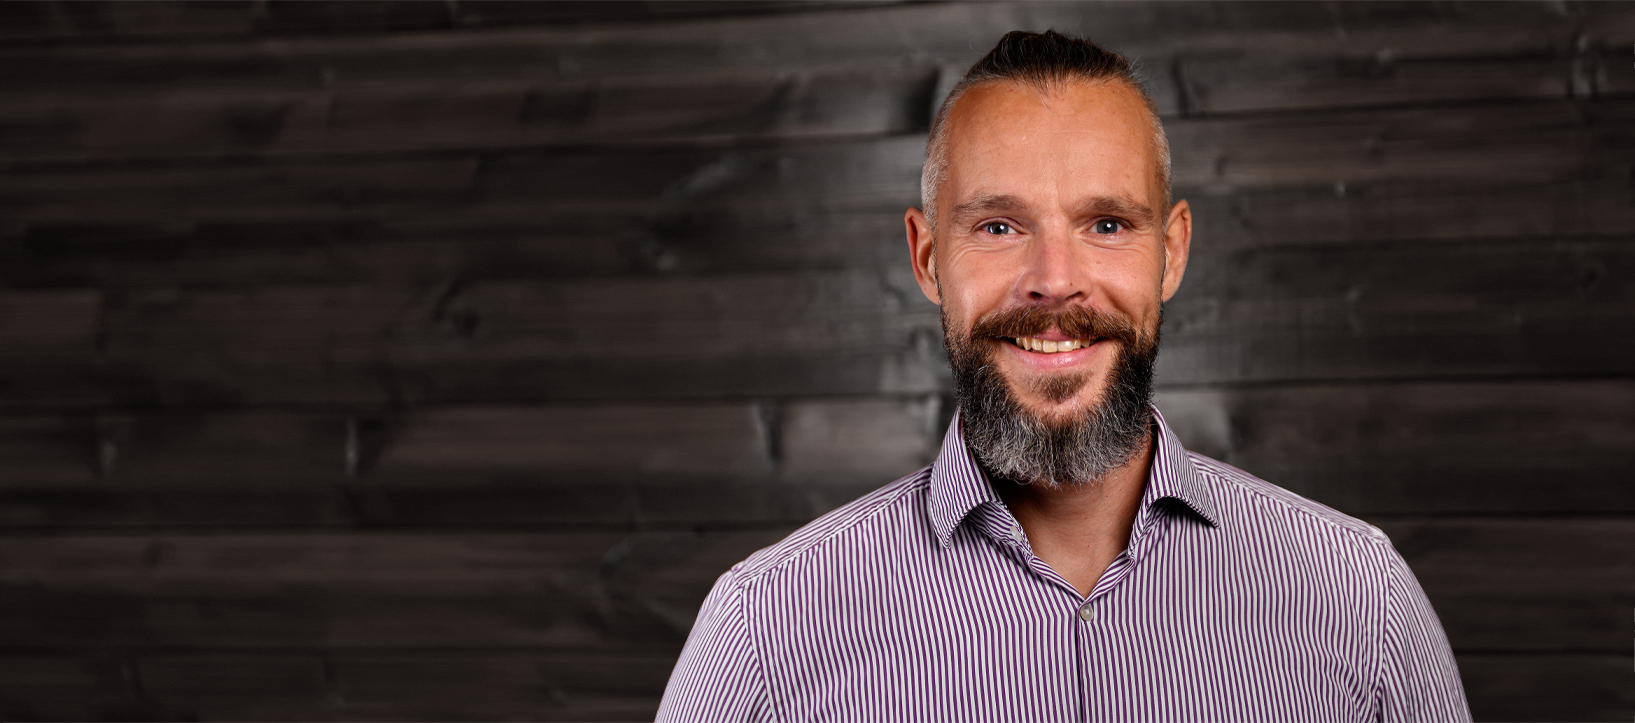
\includegraphics[trim=0 0 0 10, clip, width=\linewidth]{header.jpg}

%---------------------------------------------------------------------------------------
%	INTRODUCTION
%----------------------------------------------------------------------------------------
\pgfsetfillopacity{0.85}
\vspace{-130pt}
\hspace{0.01\linewidth}
\colorbox{msyellow}{
	\parbox{0.5\linewidth}{
		\transparent{1}
		\begin{center}
		\larrow{softcol}\textcolor{white}{
		  Passionate API designer and enthusiast about clean and robust code. Intrinsically motivated team player with a creative vein and a fondness for web design.
		}
		\end{center}
	}
}
\vspace{60pt}

%============================================================================%
%
%	CV SECTIONS AND EVENTS (MAIN CONTENT)
%
%============================================================================%

%---------------------------------------------------------------------------------------
%	SUMMARY
%----------------------------------------------------------------------------------------
\cvsection{Summary}

[ \textcolor{msgray}{\emph{Read the full detailed CV at} \href{https://cv.danieldietrich.dev}{https://cv.danieldietrich.dev}} ] \\[-2pt]

Daniel is a highly motivated Senior Software Engineer, Open Source Community Leader and Author with 18+ years of experience.
He has excellent programming skills and covers a broad range of technologies.
\\[2pt]
Daniel is passionate about API design and enthusiastic about clean and robust code.
He collaborates with developers around the world on the GitHub platform and is sharing his knowledge by writing articles and books.

\vspace{12pt}

%---------------------------------------------------------------------------------------
%	EXPERIENCE
%----------------------------------------------------------------------------------------
\cvsection{Experience}

\vspace{-1em}

\cvposition{2014 - now}{Open Source Project Leader}{\href{https://github.com/vavr-io/vavr}{Vavr} (formerly Javaslang)}
\vspace{-4pt}
\cventry{
  Reified the vision of being \#1 project for functional programming in Java.
  Built a vibrant international community and a network of open source developers and sponsors.
}

\cvposition{2008 - now}{Senior Software Engineer}{Hamburg Commercial Bank}
\vspace{-4pt}
\cventry{
  \textit{Microservice Integration Architecture for Capital Markets IT (2019-2020).}
  Designed and implemented a Capital Markets data access layer based on Open API/spec first, incl. security.
}
\cventry{
  \textit{Digital transformation of the Know Your Customer onboarding process (2018-2019).}
  Implemented an event-driven frontend in React and TypeScript that reflected updates of the onboarding process in real-time.
}
\cventry{
  \textit{Blockchain based trading platform for bonded loans (2016-2018).}
  Worked with an interdisciplinary team of German banks on the architecture and implementation of a trading platform for bonded loans.
}

\cvposition{2008}{Software Engineering Consultant}{Gentleware AG}
\vspace{-4pt}
\cventry{
  HSH Nordbank AG: \textit{Middleware for booking final taxes (2008).}
  Design and implementation of an enterprise middleware for passing payments and final taxes to multiple systems.
}

\cvposition{2002-2007}{Software Developer}{b+m Informatik AG}
\vspace{-4pt}
\cventry{
  HSH Nordbank AG: \textit{Web application for compliance (2007).}
  Created a Java client/server application to support compliance.
}
\cventry{
  UBS Germany: \textit{Reimplementation of the asset management system (2006).}
  Consultancy, requirement analysis and reimplementation of the asset management system.
}

\cvposition{1998-2002}{Student Assistant}{Inst. of Med. Inf. and Statistics}
\vspace{-4pt}
\cventry{
  Gave introductory courses about biometrics for medical students.
  Used statistics software SPSS and R.
}

\vspace{12pt}

%---------------------------------------------------------------------------------------
%	EDUCATION SECTION
%--------------------------------------------------------------------------------------
\cvsection{Education}

\vspace{-1em}

\cvposition{1997-2006}{Master's degree of Computer Science}{University of Kiel}
\vspace{-5pt}
\cventry{
  Final degree dissertation "Generator Debugging im modellgetriebenen Software-Entwicklungsprozess: Architektur und Implementierung"
}

\end{minipage}}%
\fcolorbox{white}{msblue}{\begin{minipage}[c][0.95\textheight][t]{0.33\linewidth}

%----------------------------------------------------------------------------------------
%	SIDE BAR
%----------------------------------------------------------------------------------------

\begin{metasection}{Contact}

	\icontext{MapMarker}{12}{Kiel, Germany}{white}\\[5pt]
	\icontext{MobilePhone}{12}{+49 151 645 00 968}{white}\\[5pt]
	\iconemail{Envelope}{12}{mail@danieldietrich.dev}{mail@danieldietrich.dev}{white} \\[5pt]
	\iconhref{Linkedin}{12}{linkedin.com/in/daniel-dietrich-kiel}{https://www.linkedin.com/in/daniel-dietrich-kiel/}{white} \\[5pt]
	%\iconhref{MousePointer}{12}{Webpage}{Webpage}{white} \\[5pt]
	\iconhref{Github}{12}{github.com/danieldietrich}{https://github.com/danieldietrich}{white} \\[5pt]
	%\iconhref{StackOverflow}{12}{stackoverflow.com/users/1110815/daniel-dietrich}{https://stackoverflow.com/users/1110815/daniel-dietrich}{white} \\[5pt]
	\iconhref{Twitter}{12}{@danieldietrich}{https://twitter.com/danieldietrich}{white} \\[5pt]

\end{metasection}

\vspace{-0.3cm}
\begin{metasection}{Programming Lang}\color{white}
\vspace{5pt}
\begin{tabular}{rl}

TypeScript &
\icon{Star}{12}{msyellow}\icon{Star}{12}{msyellow}\icon{Star}{12}{msyellow}\icon{Star}{12}{msyellow}\icon{Star}{12}{msyellow} \\[2pt]

JavaScript &
\icon{Star}{12}{msyellow}\icon{Star}{12}{msyellow}\icon{Star}{12}{msyellow}\icon{Star}{12}{msyellow}\icon{Star}{12}{msyellow} \\[2pt]

Java &
\icon{Star}{12}{msyellow}\icon{Star}{12}{msyellow}\icon{Star}{12}{msyellow}\icon{Star}{12}{msyellow}\icon{Star}{12}{msyellow} \\[2pt]

Bash &
\icon{Star}{12}{msyellow}\icon{Star}{12}{msyellow}\icon{Star}{12}{msyellow}\icon{Star}{12}{white}\icon{Star}{12}{white} \\[2pt]

Scala &
\icon{Star}{12}{msyellow}\icon{Star}{12}{msyellow}\icon{Star}{12}{msyellow}\icon{Star}{12}{white}\icon{Star}{12}{white} \\[2pt]

Python &
\icon{Star}{12}{msyellow}\icon{Star}{12}{msyellow}\icon{Star}{12}{white}\icon{Star}{12}{white}\icon{Star}{12}{white} \\[2pt]

Haskell &
\icon{Star}{12}{msyellow}\icon{Star}{12}{white}\icon{Star}{12}{white}\icon{Star}{12}{white}\icon{Star}{12}{white} \\[2pt]

\end{tabular}
\end{metasection}


\vspace{-0.3cm}
\begin{metasection}{Technologies}

\icontext{Code}{12}{React}{white}
\icontext{PuzzlePiece}{12}{OpenAPI}{white} \\[5pt]
\icontext{Key}{12}{oAuth \& JWT}{white}
\icontext{Database}{12}{SQL \& NoSQL}{white}


\end{metasection}


\vspace{-0.3cm}
\begin{metasection}{Tools}

\icontext{Code}{12}{VS Code}{white}
\icontext{CodeFork}{12}{Git}{white}
\icontext{Terminal}{12}{zsh}{white} \\[5pt]
\icontext{Github}{12}{GitHub}{white}
\icontext{Coffee}{12}{Coffee ;)}{white}

\end{metasection}

%---------------------------------------------------------------------------------------
%	Knowledge Areas
%----------------------------------------------------------------------------------------

\vspace{-0.3cm}
\begin{metasection}{In graphics...}
\begin{center}

\smartdiagram[bubble diagram]{
    Knowledge \\ Areas,
    \normalsize{\textbf{API design}} \\ \normalsize{\textbf{\& Tooling}},
    API\\ Security,
    \textbf{Design} \\ \textbf{Patterns},
    DevOps,
    \normalsize{\textbf{Functional}} \\ \normalsize{\textbf{Programming}},
    \textbf{SQL / NoSQL} \\ \textbf{Databases},
    \normalsize{\textbf{Web}} \\ \normalsize{\textbf{Platform}}
}

\smartdiagram[bubble diagram]{
    \normalsize{Interest} \\ \normalsize{Areas},
    \normalsize{\textbf{Algebraic}} \\ \normalsize{\textbf{Datastructures}},
    \textbf{Deep} \\ \textbf{Learning},
    \normalsize{\textbf{Efficient}} \\ \normalsize{\textbf{Algorithms}},
    \normalsize{\textbf{Graphic}} \\ \normalsize{\textbf{Design}},
    \textbf{User} \\ \textbf{Experience},
    \normalsize{\textbf{Web}} \\ \normalsize{\textbf{Design}}
}

\end{center}
\end{metasection}
\end{minipage}}

%-------------------------------------------------------------------------------------------------
%	ARTIFICIAL FOOTER (fancy footer cannot exceed linewidth)
%--------------------------------------------------------------------------------------------------

\null
\vspace*{\fill}
\hspace{-0.25\linewidth}\colorbox{msgray}{\makebox[1.5\linewidth][c]{
  \mystrut \small \textcolor{white}{
    \LaTeX~source of this \textit{résumé} is available at
    \iconhref{Github}{12}{https://github.com/danieldietrich/resume}{https://github.com/danieldietrich/resume}{white}
    ~$\cdot$~
    Last updated: \today
  }
}}

%============================================================================%
%
%	DOCUMENT END
%
%============================================================================%
\end{document}
